\documentclass{article}
\usepackage[utf8]{inputenc}
\usepackage[colorinlistoftodos,prependcaption]{todonotes}
\usepackage{graphicx}
\usepackage{hyperref}
\usepackage{listings}


\usepackage{xcolor}
\setlength\textwidth{140mm}

\lstdefinestyle{DOS}
{
    backgroundcolor=\color{gray},
    basicstyle=\color{white}\ttfamily,
    breaklines=true,
    postbreak=\mbox{\textcolor{red}{$\hookrightarrow$}\space}
}


\title{User Documentation}
\author{Socneto}
\date{February 2020}

\begin{document}

\maketitle

\section{Installation}\label{section:installation}
This section describes the installation process of the platform and its requirements. To make the installation process as simple as possible, the project can be installed using \textit{docker} and \textit{docker-compose} tools which install all the required technologies (external and internal).

\subsection{Requirements}
In order to install the platform using \textit{docker-compose} tool, the following packages are required:
\begin{itemize}
    \item \textbf{docker}, version 18.0.9.7,
    \item \textbf{docker-compose}.
\end{itemize}

The whole platform requires a minimum of 16GB of memory, but optimal is 20GB. Because many docker images need to be installed, it requires at least 20GB space on a disk.

\subsection{Installation Process}
The \textit{docker-compose} configuration is split into two files: \textit{docker-compose.yml} and \textit{docker-compose-local.yml}. The command to build, install and run the platform is the following:

\begin{lstlisting}[style=DOS]
docker-compose -f "docker-compose.yml" \
-f "docker-compose-local.yml" up
\end{lstlisting}

The command is expected to be run from the root directory of the repository. After all the docker images are started, the frontend can be found on address \textit{localhost:8080}.

\subsection{Docker Images}
In our project, we use multiple external technologies. The following list contains  all docker images which install these:

\begin{itemize}
    \item \textbf{\href{https://kafka.apache.org/}{Apache Kafka}} and its dependency \textbf{\href{https://zookeeper.apache.org/}{Apache Zookeeper}}: Kafka can be found on ports 9094 and 9092, Zookeeper can be found on port 2181,
    \item \textbf{\href{https://www.postgresql.org/}{PostgreSQL}}, which can be found on port 5432,
    \item \textbf{\href{https://www.elastic.co/}{ElasticSearch}}  version \textit{7.4.2}, running on ports 9200 and 9300,
    \item \textbf{\href{https://www.elastic.co/logstash}{Logstash}} on ports 9600, 9999 and 9998,
    \item \textbf{\href{https://www.elastic.co/kibana}{Kibana}} on port 5601.
\end{itemize}
The following list contains images that were developed within Socneto:

\begin{itemize}
    \item \textbf{Storage}: the dockerfile can be found on path \texttt{/storage/dockerfile}. It uses \textbf{\href{https://maven.apache.org/}{Maven}} image  version \textit{3.6.0} and  \textbf{\href{https://openjdk.java.net/}{OpenJDK}} image  version \textit{11} to build itself and run. After installing, it will run on port 8888,
    
    \item \textbf{Job Management Service}: the dockerfile can be found on path \\ \texttt{/job-management/Dockerfile}. It uses images \textbf{\href{https://dotnet.microsoft.com/download}{.NET Core SDK}}  version \textit{3.1} and \textbf{\href{https://dotnet.microsoft.com/apps/aspnet}{ASP.Net}}. After installing, it can be found running on port 6009,
    
    \item \textbf{Backend}: the dockerfile can be found on path \texttt{/backend/Dockerfile}. It uses images \textbf{\href{https://dotnet.microsoft.com/download}{.NET Core SDK}}  version \textit{2.2} and \textbf{\href{https://dotnet.microsoft.com/apps/aspnet}{ASP.Net}}. After installing, it can be found running on port 6010,
    
    \item \textbf{Frontend}: the dockerfile can be found on path \texttt{/frontend/Dockerfile}. It uses \textbf{Dart} version \textit{2.7.1} image to build itself and run. After installing, it can be found on port 8080,
    
    \item \textbf{Acquirers: Twitter, Reddit and Custom Static Data}: their docker files can be found in directory \texttt{/acquisition/DataAcquirer/} \\( \texttt{Dockerfile.twitter}, \texttt{Dockerfile.reddit} and \texttt{Dockerfile.customstatic}). They all use images \textbf{.NET Core SDK} version \textit{3.1} and \textbf{ASP.Net},
    
    \item \textbf{Analysers: Sentiment and Topics}: their dockerfiles can be found on paths \texttt{/analysers/sentiment\_analysis/dockerfile}\\ and \texttt{/analysers/topic\_modeling/dockerfile}. They both use \textbf{Python} image to install and run. Sentiment analyzer uses version \textit{3.7.5} while Topic analyzer uses \textit{3.8}. 
    
\end{itemize}

\subsection{Volumes}
We bind two volumes to persist data between docker builds. Directory \textbf{data01} is used to store all data from ElasticSearch, and directory \textbf{data02} is used to store all data from the PostgreSQL database.



























\section{User Documentation}

This section provides a guide on how to use Socneto platform. The user communicates with the platform via our frontend application. It is a web-based application, thus the user can use a browser to use it. If deployed using the installation process from Section \ref{section:installation}, the frontend can be found at address \textit{http://localhost:8080}. The recommended browser is Google Chrome.

\subsection{Login}
\label{section:login}

The index page (\textit{http://localhost:8080}) contains login screen. There the user needs to input correct credentials to log in and continue using the frontend. The default credentials are \textit{admin:admin}.

Additionally, the user can login only if all the core components of the platform are running. If any of them are not running, the user is informed by a warning at the bottom of login component and the login button is disabled. This can be seen in Figure \ref{figure:login}.

\begin{figure}[h]
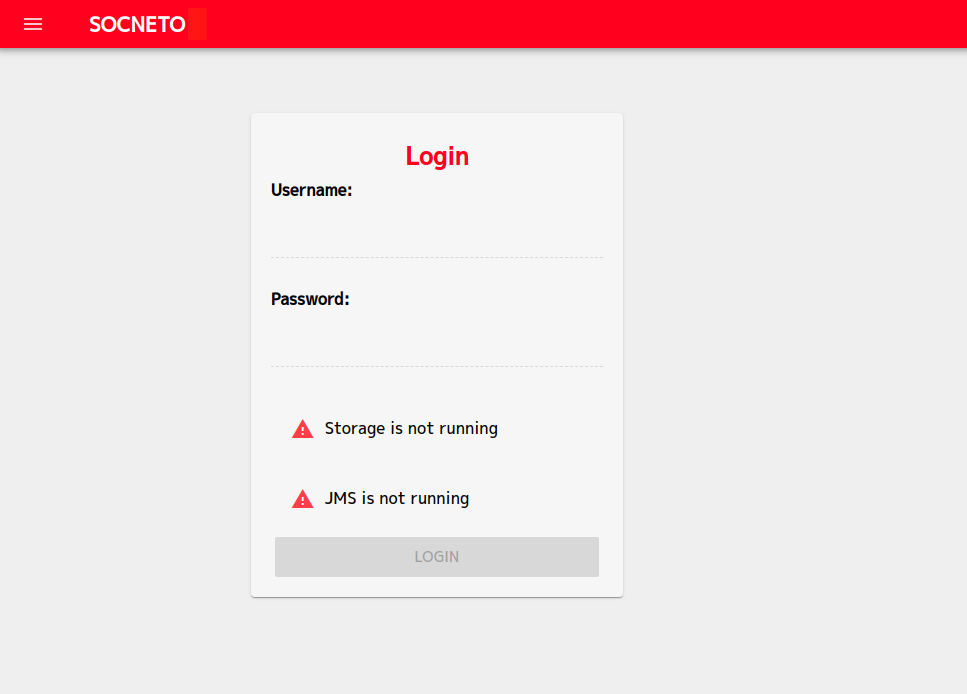
\includegraphics[width=\textwidth]{images/login.png}
\caption{Login screen when storage and job management service are not running}
\label{figure:login}
\centering
\end{figure}

\subsection{Quick Guide}

After logging in, the user is redirected to page \texttt{/\#/workspace/<username>}, where a quick guide is displayed. It is a minimal, image-based, wizard-like guide to outline the usage of the application to any user. Snapshot of the guide can be seen in Figure \ref{figure:quickguide}.

The user can navigate to the quick guide, by using \textit{Quick guide} button in the top left corner of the page. The button is displayed on every page where the user is logged in.

\begin{figure}[h]
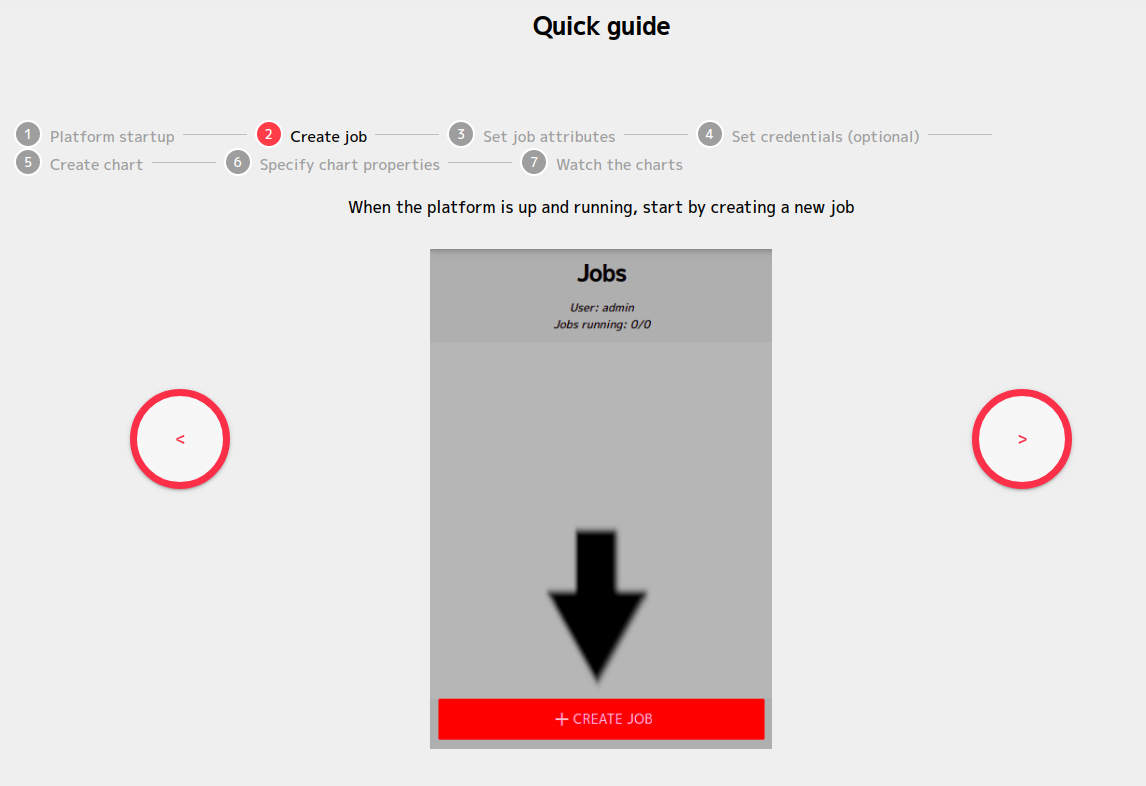
\includegraphics[width=\textwidth]{images/quick_guide.png}
\caption{Quick guide}
\label{figure:quickguide}
\centering
\end{figure}

\subsection{Platform Status}
To find out which core components of the platform are running, the user can click on \textit{hamburger menu icon} button on the left side of the page header. The button is available on all pages. It will unroll a small widget displaying the components and their status using a small colored circle next to their name. The color of the circle indicates the component's status. The colors can be:
\begin{itemize}
    \item \textbf{Green} - component is running,
    \item \textbf{Red} - component is not running,
    \item \textbf{Gray} - component's status is unknown (this happens when the backend component is not running).
\end{itemize}

The unrolled widget can be seen in Figure \ref{figure:platform-status}. Clicking anywhere outside the widget will close it.

\begin{figure}[h]
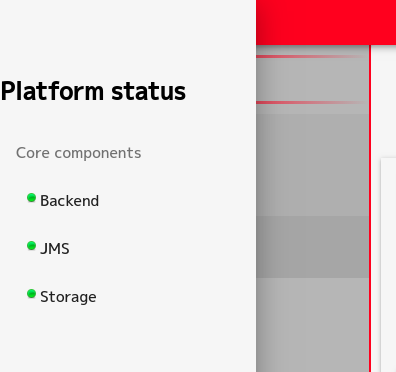
\includegraphics[scale=2.0]{images/platform_status.png}
\centering
\caption{Platform status widget}
\label{figure:platform-status}
\end{figure}

\subsection{Jobs}
One of the core activities a user can do in the frontend is creating jobs, which download data from social networks and analyze them consequently. 

\subsubsection{Jobs List}\label{section:jobs-list}
After \href{section:login}{logging in}, on page \texttt{/\#/workspace/<username>}, the user can see the list of all jobs he has created. It is displayed on the left side of the page. It also contains selected basic information about them, including title and how long they have been running. Each running job can be stopped by a stop button to the left of the job's title. When a job is stopped, it will not download any new data or analyze any new posts. 

A sample jobs list is illustrated in Figure \ref{figure:jobs-list}. It contains two running jobs called \textit{Ozzy Osbourne} and \textit{Heavy Metal}. We can see that the first one has been running for 1 day and 2 minutes, while the other for 1 day and 22 hours. We can also see the square-shaped \textit{stop button} next to each job. Above the list there is also displayed which user is logged in, and how many jobs he has created and how many of them are running. 

\begin{figure}[h]
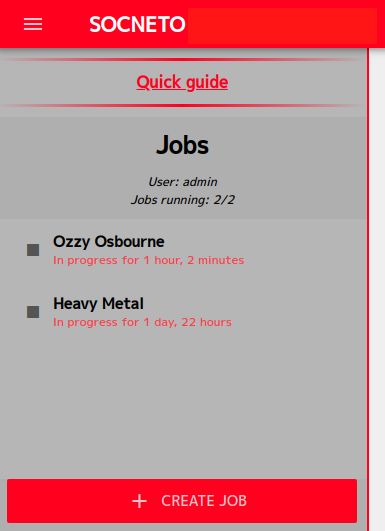
\includegraphics[scale=2]{images/jobs_list.png}
\centering
\caption{User's jobs list}
\label{figure:jobs-list}
\end{figure}

\subsubsection{Job Creation}\label{section:job-creation-dialogue}

To create a job, there is a button at the bottom part of the jobs list \textit{Create Job}, which can also be seen in Figure \ref{figure:jobs-list}. After clicking the button, a job creation dialog is shown. Similarly to the \hyperref[section:login]{login screen}, the user cannot create jobs, if any of the core components is not running. This is also displayed to the user the same way as on the \hyperref[section:login]{login screen}.

The job creation dialogue is displayed in Figure \ref{figure:create-job-dialogue}. When creating a job, the user needs to specify a few parameters of the job in the dialogue:
\begin{itemize}
  \item Title - specifies the job's title. This parameter is only for better orientation in the user's jobs list,  
  \item Topic - the topic to be queried. The topic does not need to be only one word. If multiple words are specified, the acquirers will act as if logical \textit{or} was between them, and start downloading posts, where at least one of the words is contained. To query multiple words as one topic, they need to be inside \textit{double quotes}, for example, \textit{"Star Wars"}. The topic query also supports a few logical operators, such as \texttt{; (or)}, \texttt{AND} and \texttt{NOT}, for example \texttt{humans AND elves NOT dwarves; hobbits; wizards}. This formula is then parsed into \textit{DNF} format, so it would look like \texttt{humans AND elves AND NOT dwarves AND NOT hobbits AND NOT wizards} (note the \texttt{NOT} operator being applied to the whole clause, not only the next variable),
  \item Data acquirers - select which acquirers should be used in this job. Selected acquirers will start acquiring posts for the given topic when the job is created,
  \item Data analyzers - select which analyzers should be used in this job. Selected analyzers will analyze all posts acquired by selected acquirers.
\end{itemize}
All of the above-listed parameters are required, and the job can be submitted if all of them are specified (are not empty). This can be done by clicking on the \textit{Submit} button in the dialogue. If any of these parameters is not specified, the button is disabled. This can be also seen in Figure \ref{figure:create-job-dialogue}.

\begin{figure}[h]
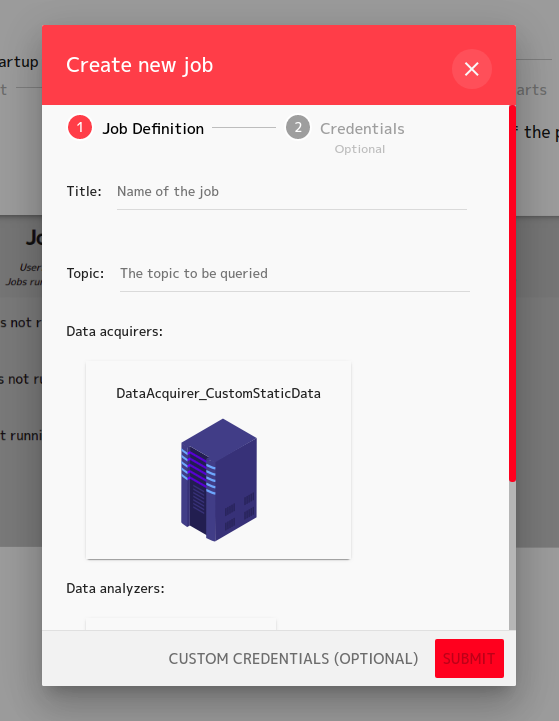
\includegraphics[scale=2]{images/create_job_dialogue.png}
\centering
\caption{Dialogue displayed when creating a job}
\label{figure:create-job-dialogue}
\end{figure}

Each of the selected acquirers can then be optionally parameterized by acquirer-specific parameters. These parameters are specified in the second step of the job creation dialogue. To get to this step, the user needs to click on the \textit{Custom credentials (optional)} button. If not all of the required parameters are specified, the button is disabled, as can be seen in Figure \ref{figure:create-job-dialogue-credential}. 

In this step, each selected acquirer has its own tab, and can be specified its own set of parameters. This can be seen in Figure \ref{figure:create-job-dialogue-credential}. In this figure, we can see three defined parameters: \texttt{bucketName}, \texttt{objectName} and \texttt{mappingName}; and their values: \texttt{example-data}, \texttt{tweets.csv} and \texttt{tweets.csv.mapping}. Which parameters the default acquirers use is described in Section \ref{section:acquirers-parameters}.

This step of job creation contains also \textit{Translate} toggle. If it is turned on, the acquired posts will be translated into English by the acquirer. The toggle can be seen in Figure \ref{figure:create-job-dialogue-credential}.

\begin{figure}[h]
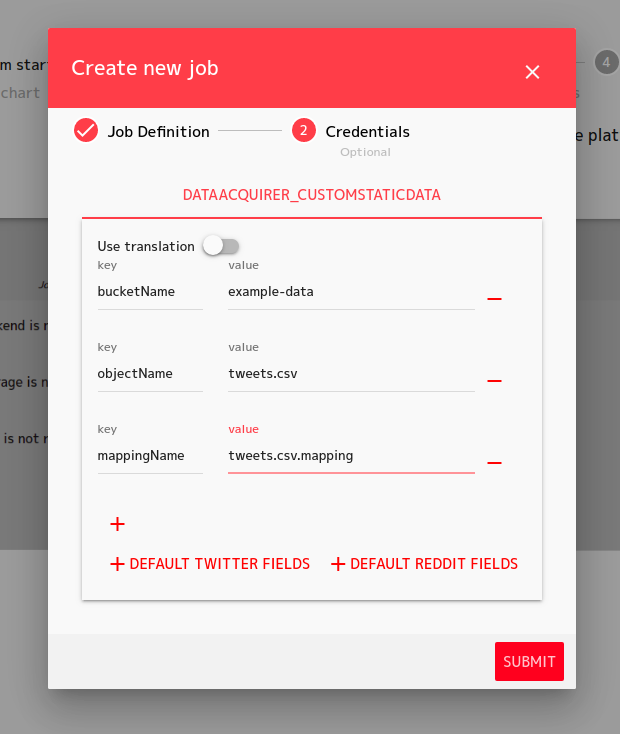
\includegraphics[scale=2]{images/create_job_credentials.png}
\centering
\caption{Optional custom credentials for acquirers}
\label{figure:create-job-dialogue-credential}
\end{figure}

\subsubsection{Acquirer's parameters} \label{section:acquirers-parameters}
Socneto comes with a few acquirers already available. These acquirers use some required or optional parameters. The following list describes these parameters:
\begin{itemize}
    \item \textbf{DataAcquirer\_Twitter} acquirer downloads tweets from \href{https://twitter.com/}{twittter.com} using its \href{https://developer.twitter.com/en/docs/api-reference-index}{API}. This API requires a user to be logged in. Thus, credentials of a user can be specified for this acquirer using the following parameters: \texttt{ApiKey}, \texttt{ApiSecretKey}, \texttt{AccessToken} and \texttt{AccessTokenSecret}. If none of them are specified, default credentials for a user with \textit{\href{https://developer.twitter.com/en/docs/basics/getting-started\#get-started-app.html}{Standard API access}} are used,
    
    \item \textbf{DataAcquirer\_Reddit} acquirer downloads posts from \href{https://www.reddit.com/}{reddit.com} using its \href{https://www.reddit.com/dev/api/}{API}. This API requires a user to be logged in. Thus, credentials of a user can be specified for this acquirer using the following parameters: \texttt{RedditAppId}, \texttt{RedditAppSecret} and \texttt{RedditRefreshToken}. If none of them are specified, default credentials for a user with free access are used,
    
    \item \textbf{DataAcquirer\_CustomStaticData} acquirer uses a \href{https://min.io/}{MinIO} server to download already acquired data. The acquirer requires parameters, which specify where the dataset files are located on the server. These parameters are \texttt{bucketName}, \texttt{objectName} and \texttt{mappingName}. More on this can be read in Section \ref{section:custom-datasets}.
\end{itemize}

\subsection{Job Data}\label{section:job-data}
After selecting a job from \href{section:jobs-list}{jobs list}, the user is redirected to page\\ \texttt{/\#/workspace/<username>/job/<jobId>}. It displays job's data. It is divided into three tabs: 
\begin{itemize}
    \item \textbf{Detail} - displays some basic information and analyses for the job (more in Section \ref{section:job-detail}),
    \item \textbf{Analyses} - displays user defined charts of analyses of job's acquired posts (more in Section \ref{section:job-analyses}),
    \item \textbf{Posts} - displays list of all acquired posts by the job (more in Section \ref{section:job-posts}.
\end{itemize}

These tabs can be seen on the top of Figure \ref{figure:job-detail}. This page also displays \href{section:jobs-list}{jobs list} on the left side.

\subsection{Job Detail}\label{section:job-detail}
The first tab in job's data page (Section \ref{section:job-data}) displays basic information about the job, such as: \textit{topic query} (as specified during job creation), \textit{status} (running or stopped), \textit{posts count} (number of posts acquired by acquirers for the current job), \textit{date} when the job was started and its \textit{running time}. These are displayed on the very top of the page, as can be seen in Figure \ref{figure:job-detail}.

Following this information, some basic analyses are displayed. These analyses are: 
\begin{itemize}
    \item \textbf{Posts frequency} - line chart whose x-axis is time (split into hour long interval) and y-axis is number of posts acquired for given hour (can be seen in Figure \ref{figure:job-detail}),
    \item \textbf{Language frequency} - table displaying languages (in \textit{ISO 3166 Alpha-2 format}) and how many acquired posts were written in given language,
    \item \textbf{Author frequency} - table displaying authors and how many acquired posts were posted by given author.
\end{itemize}

\begin{figure}[h]
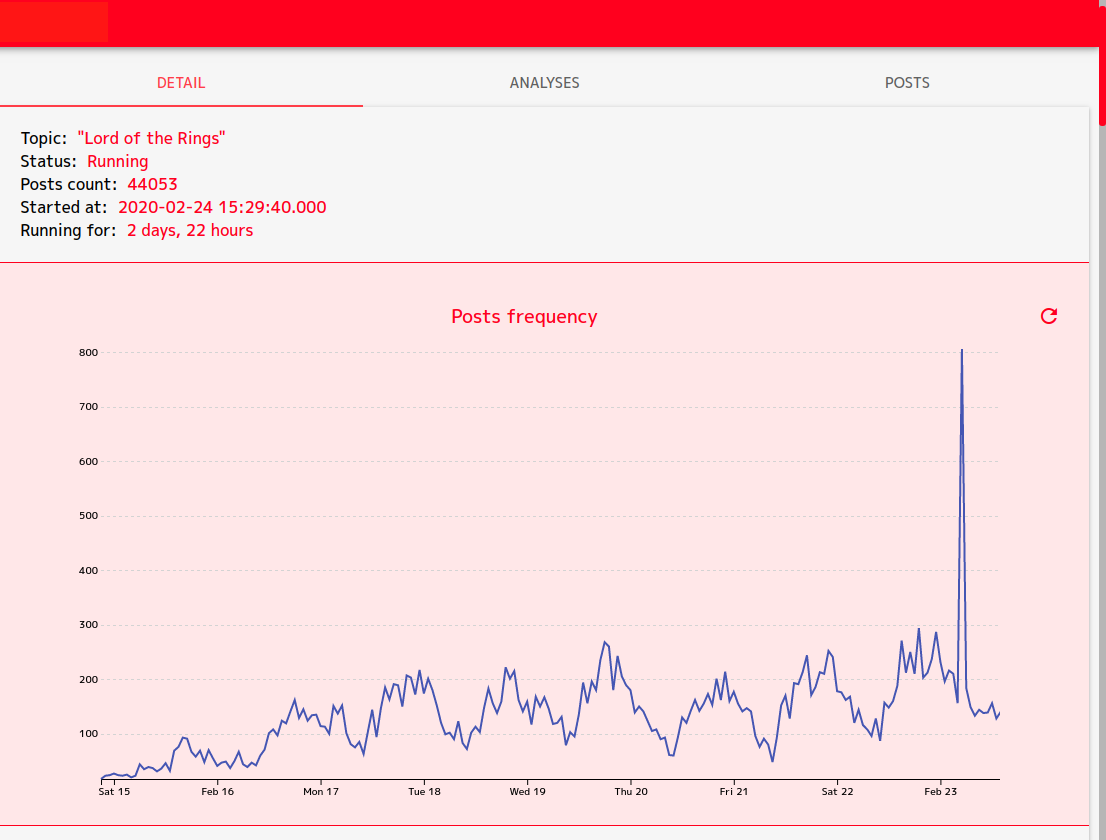
\includegraphics[width=\textwidth]{images/job_detail.png}
\centering
\caption{Example of a job detail tab}
\label{figure:job-detail}
\end{figure}

\subsection{Charts}\label{section:job-analyses}
The second tab in the job's data page (Section \ref{section:job-data}) displays user-defined charts of downloaded posts' analyses. The user can create any number of charts for any \textit{running or stopped} job. Which data is displayed in the chart depends entirely on the user's specification of the chart. A user-defined chart called \textit{Topics - pie} can be seen in Figure \ref{figure:pie-chart}.

\subsubsection{Chart Creation}
At the bottom of the charts list is a large '\textit{+}' button. Clicking it will show a chart creation dialogue. The dialogue can be seen in Figure \ref{figure:create-chart-dialogue}. The chart creation process differs slightly for different types of charts. The user is required to specify the following parameters:
\begin{itemize}
    \item \textbf{Chart title} - used only for user's better orientation in the list of charts,
    \item \textbf{Chart type} - select from five different types of chart: \textit{line chart}, \textit{pie chart}, \textit{bar chart}, \textit{table}, \textit{word cloud} and \textit{scatter chart}, 
    \item \textbf{Analyses' properties} - specify which properties from analyzers should be displayed in the charts:
    \begin{itemize}
        \item \textbf{Line chart} - the x-axis of the line chart can be either a numeric property from posts' analyses or posts' posted time. This can be specified by checking or unchecking \textit{Use post time on X axis} checkbox. If it is unchecked, the \textit{X-Axis} analysis property must be specified. Either way, at least \textit{Line 1} analysis property must be specified, and consequently, any number of following lines can be specified,
        \item \textbf{Pie chart, Bar chart, Word cloud and Table} - only one analysis property can be specified for these types of charts. The values of this analysis property are then aggregated over all the acquired posts and shown in the charts,
        \item \textbf{Scatter chart} - exactly two analysis properties must be specified for this type of chart. The first one is used for the x-axis, and the second one for the y-axis. The scatter chart is then created according to the values of theses analysis properties appearing in the acquired posts.
    \end{itemize}
\end{itemize}.
Not all analyzers' output fields can be displayed by all charts. Line and scatter charts are able to display only numeric field. Pie, bar and table charts can display only map and list fields. Word cloud can display only map and list of text fields. More on analyzers' output fields can be found in \textit{Development documentation} document, in Section \textit{3.7.5 Communication}.

This dialogue can be seen in Figure \ref{figure:create-chart-dialogue}, where pie chart type is selected, and the selected property to be aggregated in the chart is \textit{topics} from analyzer \textit{DataAnalyser\_topics}.

\begin{figure}[h]
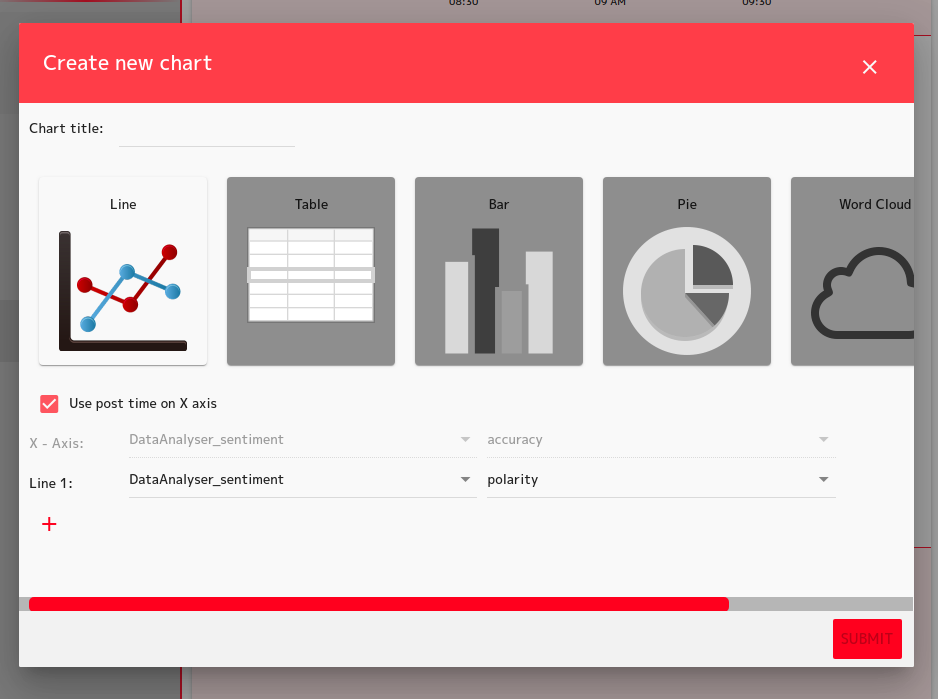
\includegraphics[width=\textwidth]{images/chart_creation_dialogue.png}
\centering
\caption{Chart creation dialogue with line chart type and sentiment analysis property selected}
\label{figure:create-chart-dialogue}
\end{figure}

\subsection{Charts List}
The charts in the charts list are not updated automatically as new analyses arrive in the platform. However, they can be refreshed by clicking on the \textit{bent arrow} button in the top-right corner of the chart's widget. There is also a \textit{trash} button which removes the chart entirely. These buttons can be seen on the top right corner of Figure \ref{figure:pie-chart}.

Some of the slices of \textit{Pie chart} may be so small, that their labels are written over each other. To highlight any of the slice labels, mouse hover over the slice. This is illustrated in Figure \ref{figure:pie-chart}.

\begin{figure}[h]
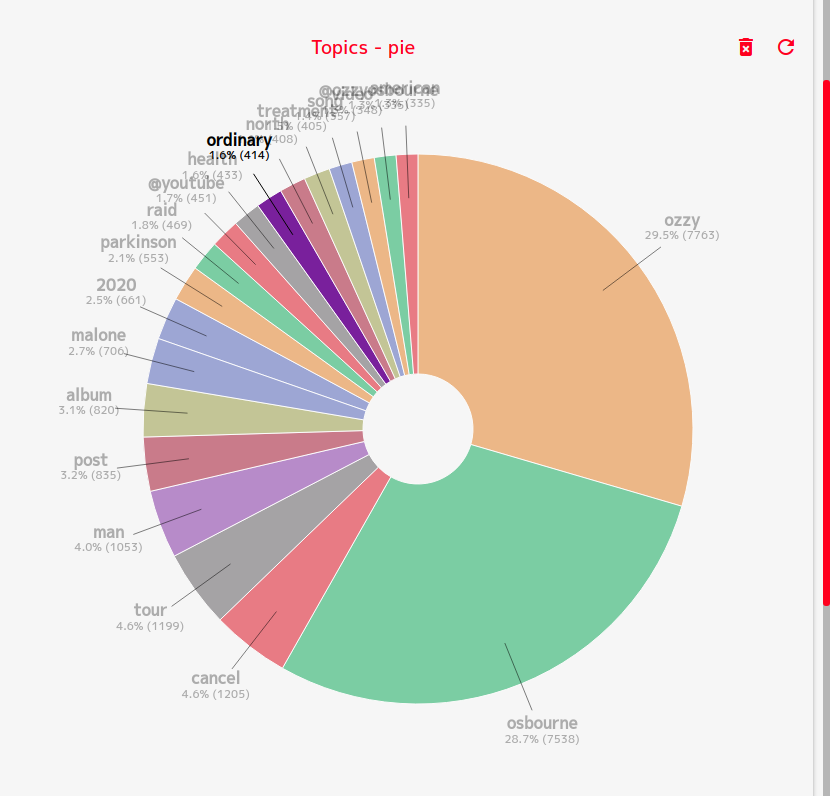
\includegraphics[width=\textwidth]{images/pie_chart.png}
\centering
\caption{Highlighting one of pie chart's slices}
\label{figure:pie-chart}
\end{figure}

If there is a large amount of data, line charts cannot show them all at once and they become paginated. When this happens, buttons to move the chart forward or backward on the x-axis will appear to the right and left of the chart. This can be seen in Figure \ref{figure:line-chart-pagination}.

\begin{figure}[h]
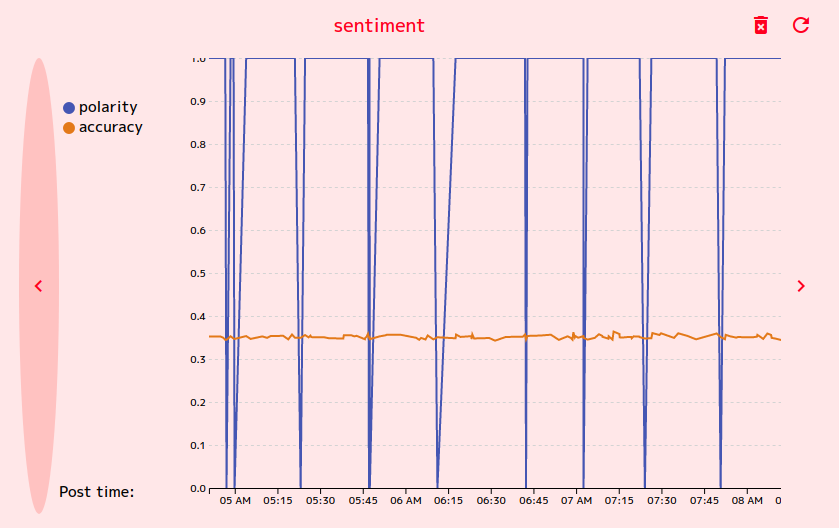
\includegraphics[width=\textwidth]{images/line_chart.png}
\centering
\caption{Line chart with 'forward' and 'backward' buttons on the sides}
\label{figure:line-chart-pagination}
\end{figure}

\subsection{Posts}\label{section:job-posts}
The third tab in job's data page (Section \ref{section:job-data}) displays all acquired posts of the job. This list can be seen in Figure \ref{figure:posts-list}. Since there will mostly be a large number of these posts, they are paginated, displaying 20 posts in one page. They can also be filtered out by three criteria:
\begin{itemize}
    \item Date range - specify a date range, from which the filtered posts should be picked. The filtered posts will be then picked from the 0:00 of the beginning date to the 23:59 of the ending date,
    \item Contain words - specify words, from which at least one must be contained in the filtered posts,
    \item Exclude words - specify words that the filtered posts can't contain.
\end{itemize}

The posts are updated automatically as the filters are updated. However, as well as charts, they are not updated automatically as new posts arrive in the platform. They can be refreshed by clicking on the \textit{bent arrow} button in the top-right corner of the posts list. The button can be seen on the top right part of Figure \ref{figure:posts-list}.

\begin{figure}[h]
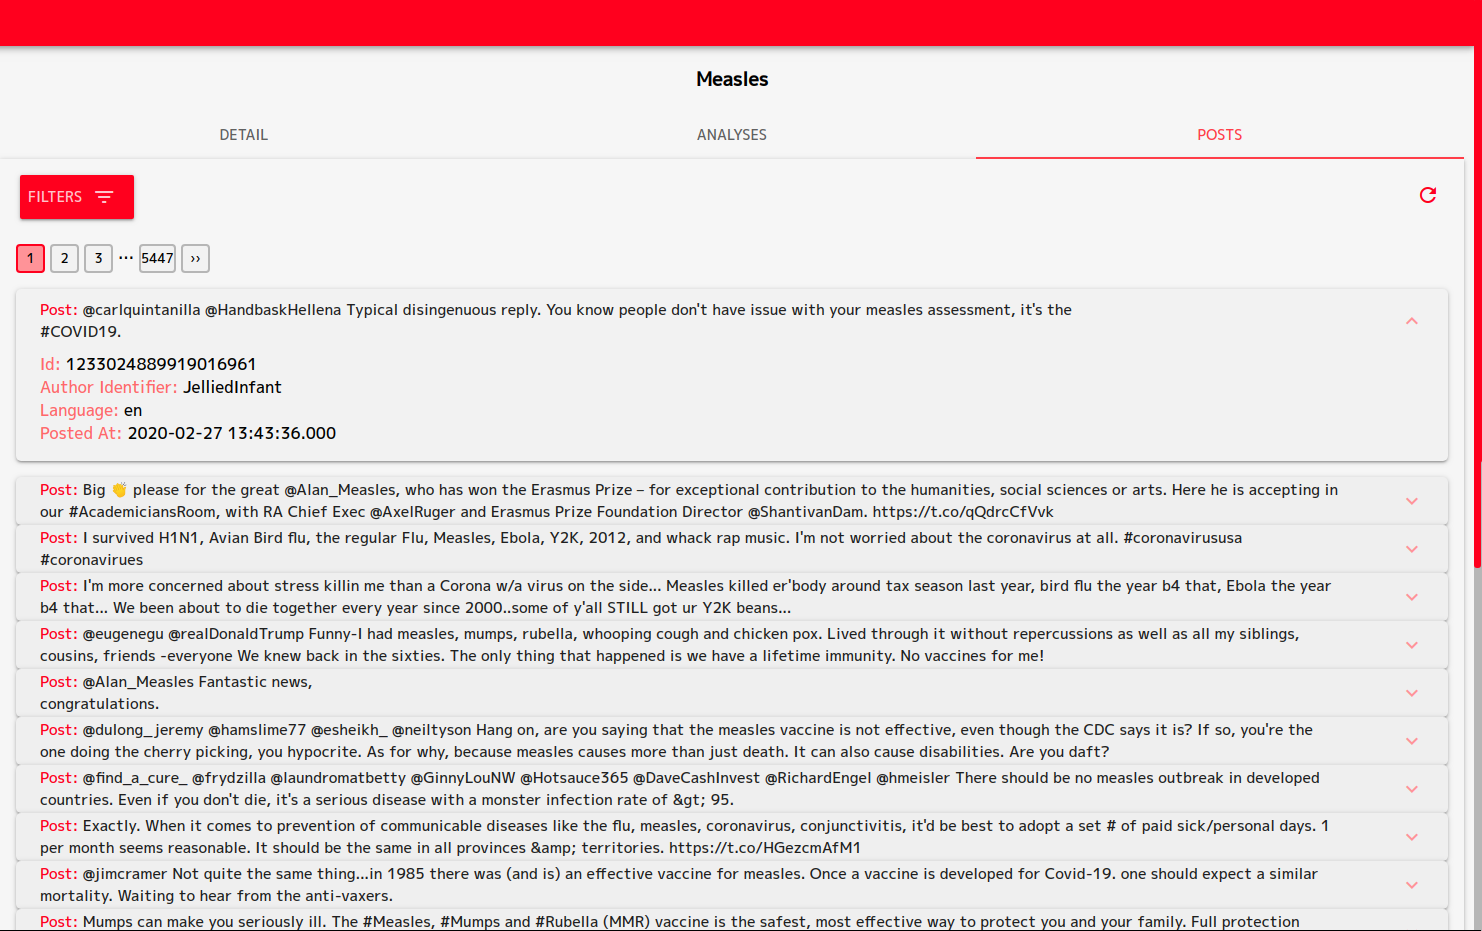
\includegraphics[width=\textwidth]{images/posts_list.png}
\centering
\caption{Illustration of filtered posts list with some posts' detail unrolled}
\label{figure:posts-list}
\end{figure}

\subsubsection{Post Detail}\label{section:post-detail}
Any of the posts can be clicked on, to unroll more information about it. Only properties that are available are displayed. These properties are: \textit{post's original identifier}, \textit{post's original text} (if it was translated by the acquirer), \textit{language} (in \textit{ISO 3166 Alpha-2 format}) of the post, \textit{identifier of author} of the post and \textit{date} at which the post was posted. This is also illustrated in Figure \ref{figure:posts-list}. There, the very first post is unrolled, showing its properties.

\subsubsection{Export}
These (un)filtered posts can be also exported into CSV format file by pressing button \textit{Export to CSV} located at the bottom of the posts list. It is displayed only if the list contains at least one post. 

The exported CSV contains all the posts, not only posts from the currently displayed page. It contains all the attributes mentioned in Section \ref{section:post-detail}.


\section{Advanced User Documentation}
Next to using only frontend, Socneto platform has several advanced features:
\begin{itemize}
    \item Using custom data set for analyses,
    \item Adding custom analyzer or acquirer
\end{itemize}

\subsection{Custom Datasets}\label{section:custom-datasets}
Socneto allows users to use their own datasets as long as they comply with the following requirements.

\begin{itemize}
    \item \textbf{File format} - supported file formats are \texttt{csv} and \texttt{json}. In case of json, the file is assumed to be in \texttt{json line} format, where each line is a json record. We will refer to this format as to plain \texttt{json},
    \item \textbf{Content} must be transformable into an entity \texttt{Post}. The transformation is done via mapping file accompanying the dataset.
\end{itemize}

\subsubsection{Dataset Transformation}
The components processing data from custom dataset expect each record to have the following fields:

\begin{itemize}
    \item \texttt{originalPostId} - a unique post string identifier (for example \texttt{1234abcd-efgh}),
    \item \texttt{text} - the text of the given post,
    \item \texttt{language} - the language code of the post (ISO 3166 Alpha-2 format).  The post be in any language, but only sentiment of English posts can be analysed. Example: \texttt{en}, \texttt{cs} or \texttt{null},
    \item \texttt{source} - field prefilled by the Data acquirer. Example: \texttt{twitter\_acquirer},
    \item \texttt{authorId} - the name or id of the author. Can be \texttt{null},
    \item \texttt{dateTime} - date time when the post was created (in ISO8601 format). Example: \texttt{2020-01-03T23:42:53}
\end{itemize}

Socneto implements basic automatic transformation that maps records from the dataset to the \texttt{Post} format. The transformation requires a json configuration file specifying:

\begin{itemize}
    \item \textbf{mapping} of fields from dataset records to \texttt{Post},
    \item \textbf{specification} of fixed values (e.g. language may be the same across the dataset or the value is not present),
    \item \textbf{file format} - either `csv` or `json`,
    \item  \textbf{format specific} configuration
\end{itemize}

The mapping configuration files have the following  fields:

\begin{itemize}
    \item \texttt{dataFormat} - format of the dataset, \texttt{json} or \texttt{csv}. This field is required,
    \item \texttt{mappingAttributes} - root element with mappings and element specific values. This field is required,
    \item \texttt{fixedValues} - map where a key is a name of a field of the \texttt{Post} entity and the value is a text of the field. This field is not required,
    \item \texttt{indices} (for \texttt{csv} data format only) - map where a key is  a name of a field of the \texttt{Post} entity and value is an index of the record with target value. Required for \texttt{csv} file format,
    \item \texttt{elements} (for \texttt{json} data format only) - map where a key is  a name of a field of the \texttt{Post} entity and value is a name of an element of the record with target value. Mapping to names of csv columns is not supported, use \texttt{indices} instead. Required for \texttt{json} file format,
    \item \texttt{hasHeaders} - indication whether the \texttt{csv} file contains headers or not (they will be skipped if true). Required for \texttt{csv} file format,
    \item \texttt{dateTimeFormatString} - if dateTime mapping is specified, then this field is used as mask for custom date time formats. If no format string is specified then \hyperref[https://docs.microsoft.com/en-us/dotnet/api/system.datetime.tryparse?view=netcore-3.1]{the default one} is used. This field is not required.
\end{itemize}

\subsubsection{JSON Mapping File Example}
\begin{lstlisting}
{
    "dataFormat":"json",
    "mappingAttributes":{
        "hasHeaders":true,
        "dateTimeFormatString":"yyyy'-'MM'-'dd'T'HH':'mm':'ss",
        "fixedValues":{
            "language":"en"
        },
        "elements":{
            "originalPostId":"PostId",
            "text":"Text",
            "authorId":"UserId",
            "dateTime":"PostDateTime"
        }
    }
}
\end{lstlisting}

This file is used to map the following json record:

\begin{lstlisting}
{
    "PostId":"1195555506847744",
    "Text":"The movie xyz was excelent",
    "UserId":"abc",
    "PostDateTime":"2019-11-16T18:48:03"
}
\end{lstlisting}

The resulting \texttt{Post} (shown in json) is the following:
\begin{lstlisting}
{
    "originalPostId":"1195555506847744",
    "text":"The movie xyz was excelent",
    "source":"twitter_acquirer", // filled with the acqurier
    "authorId":"abc",
    "dateTime":"2019-11-16T18:48:03",
    "language":"en"
}
\end{lstlisting}

\subsubsection{CSV Mapping File Example}\label{section:csv-mapping-file}
\begin{lstlisting}
{
    "dataFormat":"csv",
    "mappingAttributes":{
        "hasHeaders":true,
        "dateTimeFormatString":"ddd MMM dd HH:mm:ss PDT yyyy",
        "fixedValues":{
            "language":"en"
        },
        "indices":{
            "originalPostId":1,
            "text":5,
            "authorId":4,
            "dateTime":2
        }
    }
}
\end{lstlisting}

This mapping file is used to map the following record (in csv format):

\begin{lstlisting}
target,id,date,flag,user,text
0,abd087, Sat May 16 23:58:44 UTC 2008,xyz,robotickilldozr,xyz is fun
\end{lstlisting}

The resulting \texttt{Post} (shown in json) is the following:

\begin{lstlisting}
{
    "originalPostId":"abc087",
    "text":"xyz is fun",
    "source":"twitter_acquirer", // filled with the acqurier
    "authorId":"abc",
    "dateTime":"2009-05-16T23:58:44",
    "language":"en",  
}
\end{lstlisting}

\textbf{CAUTION:} When parsing of the date time is not successful, then the \texttt{dateTime} field of the resulting \texttt{Post} entity is set to `0001-01-01T00:00:00`.

\textbf{NOTE:} Mappings do not support any nested json files. If user needs so, then there is a possibility to extend the system with own implementation supporting such a mapping.

When transformation fails to produce valid \texttt{Post} object then the object is not produced and will be ignored. User is noticed about the problem with a warning message that can be found in the logs.


\subsubsection{Full Example of Adding Custom Dataset}
The following text works with \href{https://www.kaggle.com/kazanova/sentiment140}{this dataset} that can be found on \href{https://www.kaggle.com}{kaggle.com}. The dataset will be referred to as \texttt{tweets.csv}. It is a single \texttt{csv} file with 1.6 million records with the following columns:

\begin{itemize}
    \item \texttt{target} - the polarity of the tweet e.g. 0 = negative, 2 = neutral, 4 = positive,
    \item \texttt{id} - the id of the tweet,
    \item \texttt{date} - the date when the tweet was tweeted,
    \item \texttt{flag} - the query which was used to obtains the given tweet. If there is no query, then this value is NO\_QUERY,
    \item \texttt{user} - the user that tweeted the tweet,
    \item \texttt{text} - the content of the tweet.
\end{itemize}

The mapping configuration file used (referred to as \texttt{tweets.mapping}) is the same as was presented in the Section \ref{section:csv-mapping-file}. The following steps lead to successfully feeding Socneto with these data.

\begin{enumerate}
    \item \textbf{Upload files} - connect to \texttt{http://acheron.ms.mff.cuni.cz:39111} and login with the following credentials: username \texttt{socnetoadmin}, password \texttt{Tajn0Heslo}. After logging in hit red plus button and create bucket \texttt{movie-tweets}. Hit the upload button again and upload \texttt{tweets.csv} and \texttt{tweets.mapping} to that bucket. After this step, you should see the screen like in Figure \ref{figure:minio-uploads},
    \item \textbf{Create a job} - create a new job via frontend, using process described in Section \ref{section:job-creation-dialogue}. Use acquirer called \texttt{DataAcquier\_CustomStaticData}.
\end{enumerate}

\begin{figure}[h]
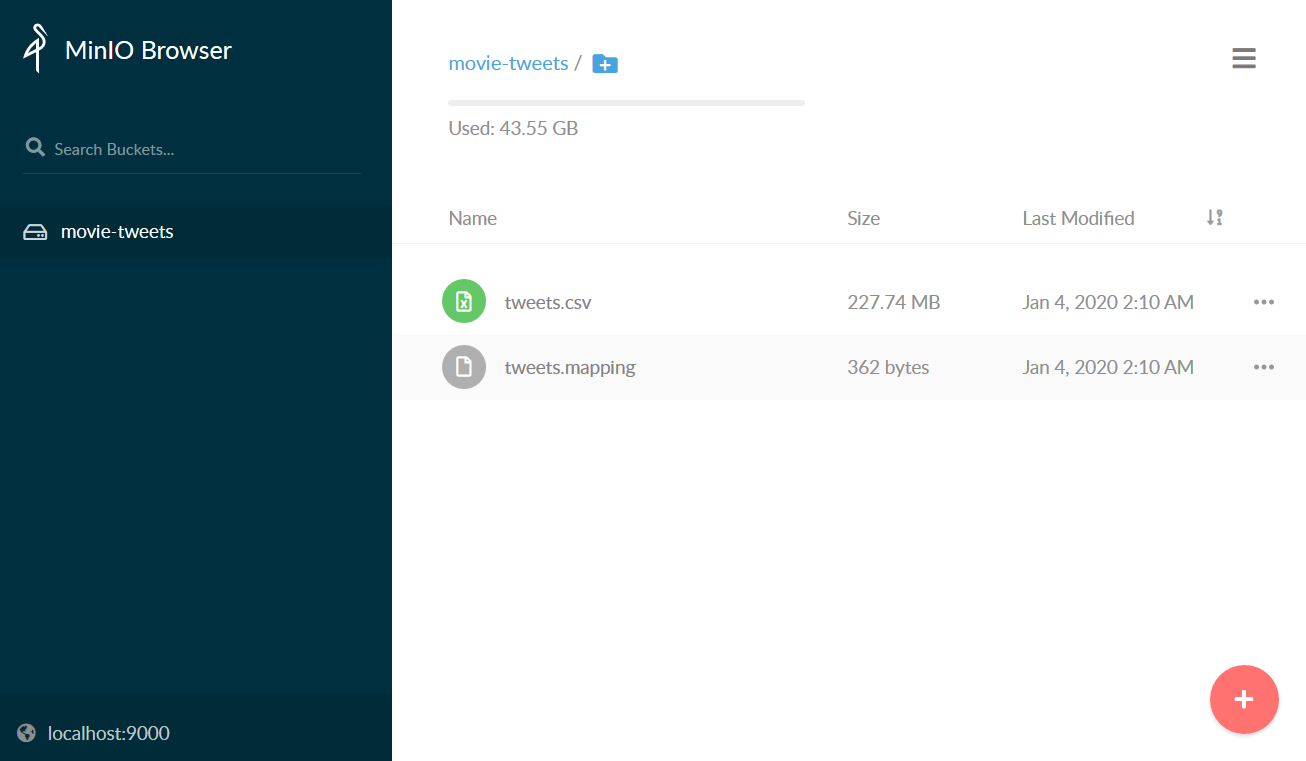
\includegraphics[width=\textwidth]{images/minio_files.png}
\centering
\caption{Example of files uploaded to minio server}
\label{figure:minio-uploads}
\end{figure}

\subsection{Custom Acquirers and Analyzers}
The process of implementing custom acquirers and analyzers is thoroughly described in \textit{Development Documentation} in \textit{Section 3.10 Extensibility}.

If a new component is correctly implemented and started, it will be displayed in the job creation dialogue from Section \ref{section:job-creation-dialogue}.

\end{document}
